% coding:utf-8

%FOSALRS, a LaTeX-Code for a electrical summary of control theory
%Copyright (C) 2013, Daniel Winz, Ervin Mazlagic

%This program is free software; you can redistribute it and/or
%modify it under the terms of the GNU General Public License
%as published by the Free Software Foundation; either version 2
%of the License, or (at your option) any later version.

%This program is distributed in the hope that it will be useful,
%but WITHOUT ANY WARRANTY; without even the implied warranty of
%MERCHANTABILITY or FITNESS FOR A PARTICULAR PURPOSE.  See the
%GNU General Public License for more details.
%----------------------------------------

\chapter{Signale}
\newpage

\section{Einheitssprung}
Die Sprungfunktion $\sigma(t)$ (auch \emph{Einheitssprung}) ist eine
Funktion, welche definiert ist als
\[ 
    \sigma(t) := 
    \left\{
        \begin{array}{c c}
            1 & t \geq 0 \\
            0 & t \leq 0
        \end{array}
    \right.
\]
\begin{figure}[h!]
    \centering
    \begin{tikzpicture}
        % zeichne Koordinatensystem
        \draw[->] (-2,0) -- (4,0) node[anchor=north] {$t$};
        \draw[->] (0,0) -- (0,2) node[anchor=east] {$\sigma(t)$};

        % zeichne Labels
        \draw (0,0) node[anchor=north] {$0$};
        \draw (0,1) node[anchor=east] {$1$};

        % Zeigne Singalverlauf
        \draw[-, thick, red] (-1.5,0) -- (0,0) {};
        \draw[-, thick, red] (0,0) -- (0,1) {};
        \draw[-, thick, red] (0,1) -- (3.5,1) {};
    \end{tikzpicture}
    \caption{Sprungfunktion}
    \label{fig:sprungfunktion}
\end{figure}
Diese allgemeine Definition kann verwendet werden um die Funktion für
ein Signal anzupassen. Beispielsweise kann die Amplitude 1 mit einem
reellen Faktor $A$ multipliziert oder die Sprungstelle bei $t=0$ um
$t_1$ verschoben werden.
\[  
        u(t) = A \cdot \sigma(t-t_1)
\]
\begin{figure}[h!]
    \centering
    \begin{tikzpicture}
        % zeichne Koordinatensystem
        \draw[->] (-2,0) -- (4,0) node[anchor=north] {$t$};
        \draw[->] (0,0) -- (0,2) node[anchor=east] {$u(t)$};

        % zeichne Labels
        \draw (0,0) node[anchor=north] {$0$};
        \draw (0,1) node[anchor=east] {$A$};
        \draw (1,0) node[anchor=north] {$t_1$};

        % Zeichne Singalverlauf
        \draw[-, thick, red] (-1.5,0) -- (1,0) {};
        \draw[-, thick, red] (1,0) -- (1,1) {};
        \draw[-, thick, red] (1,1) -- (3.5,1) {};
    \end{tikzpicture}
    \caption{Sprungfunktion mit
        $u(t) = A \cdot \sigma(t-t_1)$}
    \label{fig:sprungfunktion2}
\end{figure}

\section{Rampe}
\[ 
    u(t) = 
    \left\{
        \begin{array}{c c}
            t & t \geq 0 \\
            0 & t < 0
        \end{array}
    \right.
    = t \cdot \sigma(t)
\]
\begin{figure}[h!]
    \centering
    \begin{tikzpicture}
        % zeichne Koordinatensystem
        \draw[->] (-2,0) -- (4,0) node[anchor=north] {$t$};
        \draw[->] (0,0) -- (0,2) node[anchor=east] {$u(t)$};

        % zeichne Labels
        \draw (0,0) node[anchor=north] {$0$};

        % Zeigne Singalverlauf
        \draw[-, thick, red] (-1.5,0) -- (0,0) {};
        \draw[-, thick, red] (0,0) -- (3.5,1.5) {};
    \end{tikzpicture}
    \caption{Rampenfunktion}
    \label{fig:rampenfunktion}
\end{figure}

\section{Rechteckimpuls}
\[ 
    u(t) = 
    \left\{
        \begin{array}{c c}
            A & t_0 \leq t \leq t_1 \\
            0 & t_1 < t < t_0
        \end{array}
    = A \cdot (\sigma(t - t_0) - \sigma(t - t_1))
    \right.
\]

\begin{figure}[h!]
    \centering
    \begin{tikzpicture}
        % zeichne Koordinatensystem
        \draw[->] (-2,0) -- (4,0) node[anchor=north] {$t$};
        \draw[->] (0,0) -- (0,2) node[anchor=east] {$u(t)$};

        % zeichne Labels
        \draw (0,0) node[anchor=north] {$t_0$};
        \draw (2,0) node[anchor=north] {$t_1$};
        \draw (0,1) node[anchor=east] {$A$};

        % Zeigne Singalverlauf
        \draw[-, thick, red] (-1.5,0) -- (0,0) {};
        \draw[-, thick, red] (0,0) -- (0,1) {};
        \draw[-, thick, red] (0,1) -- (2,1) {};
        \draw[-, thick, red] (2,1) -- (2,0) {};
        \draw[-, thick, red] (2,0) -- (3.5,0) {};
    \end{tikzpicture}
    \caption{Rechteckimpuls}
    \label{fig:rechteckimpuls}
\end{figure}


\section{Dirac}
Die Dirac-Delta Funktion $\delta(t)$ ist das Ergebnis der abgeleiteten
Sprungfunktion $\sigma(t)$.
\[  
    \delta(t) =
    \dot{\sigma}(t) =
    \left\{ 
        \begin{array}{c c}
            \infty & t=0 \\
            0 & t \neq 0
        \end{array}
    \right.
\]
Die Herleitung der Dirac-Delta Funktion ist anschaulich mittels eines
Plots der Sprungfunktion. Nähert man eine Funktion an den Verlauf der
Sprungfunktion an, so ergibt deren Ableitung eine Rechteckfunktion.
Die Fläche $A$ unter dem Rechteck ist dabei stets $1$.
\[ 
    \widetilde{\sigma}(t, \Delta t) = 
    \left\{
        \begin{array}{c c}
            1 & t > \Delta t \\
            \frac{1}{2} + \frac{t}{2 \cdot \Delta t} &
            - \Delta t \leq t \leq \Delta t \\
            0 & t < - \Delta t
        \end{array}
    \right.
\]
\begin{figure}[h!]
    \centering
    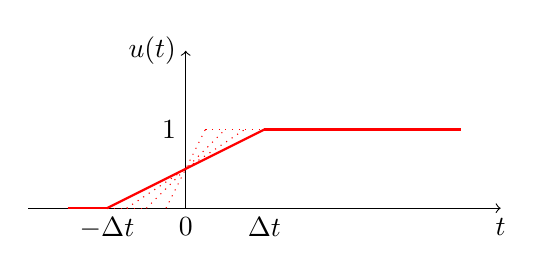
\begin{tikzpicture}
        % zeichne Koordinatensystem
        \draw[->] (-2,0) -- (4,0) node[anchor=north] {$t$};
        \draw[->] (0,0) -- (0,2) node[anchor=east] {$u(t)$};

        % zeichne Labels
        \draw (0,0) node[anchor=north] {$0$};
        \draw (0,1) node[anchor=east] {$1$};
        \draw (-1,0) node[anchor=north] {$- \Delta t$};
        \draw (1,0) node[anchor=north] {$\Delta t$};

        % Zeigne Singalverlauf
        \draw[-, thick, red] (-1.5,0) -- (-1,0) {};
        \draw[-, thick, red] (-1,0) -- (1,1) {};
        \draw[-, thick, red] (1,1) -- (3.5,1) {};

        %\draw[-, red, dotted] (-1.5, 0) -- (-0.75, 0) {};
        \draw[-, red, dotted] (-0.75, 0) -- (0.75, 1) {};
        %\draw[-, red, dotted] (0.75, 1) -- (3.5, 1) {};

        %\draw[-, red, dotted] (-1.5, 0) -- (-0.5, 0) {};
        \draw[-, red, dotted] (-0.5, 0) -- (0.5, 1) {};
        %\draw[-, red, dotted] (0.5, 1) -- (3.5, 1) {};

        \draw[-, red, dotted] (-1.5, 0) -- (-0.5, 0) {};
        \draw[-, red, dotted] (-0.25, 0) -- (0.25, 1) {};
        \draw[-, red, dotted] (0.25, 1) -- (3.5, 1) {};
    \end{tikzpicture}
    \caption{Dirac-Delta Funktion}
    \label{fig:dirac-delta}
\end{figure}
\[      
    \frac{d \widetilde{\sigma}(t)}{dt} = 
    \left\{
        \begin{array}{c c}
            0 & t > \Delta t \\
            \frac{1}{2 \cdot \Delta t} &
            - \Delta t \leq t \leq \Delta t \\
            0 & t < - \Delta t
        \end{array}
    \right.
\]
\begin{figure}[h!]
    \centering
    \begin{tikzpicture}
        \usepgflibrary{patterns}
        % zeichne Koordinatensystem
        \draw[->] (-2,0) -- (4,0) node[anchor=north] {$t$};
        \draw[->] (0,0) -- (0,2) node[anchor=east] {$u(t)$};

        % zeichne Labels
        \draw (0,0) node[anchor=north] {$0$};
        \draw (-1,1) node[anchor=east] {$\frac{1}{2 \cdot \Delta t}$};
        \draw (-1,0) node[anchor=north] {$- \Delta t$};
        \draw (1,0) node[anchor=north] {$\Delta t$};

        % Fläche einfärben
        \draw[pattern=north east lines, pattern color=gray]
            (-1,0) rectangle (1,1);

        % Zeigne Singalverlauf
        \draw[-, thick, red] (-1.5,0) -- (-1,0) {};
        \draw[-, thick, red] (-1,0) -- (-1,1) {};
        \draw[-, thick, red] (-1,1) -- (1,1) {};
        \draw[-, thick, red] (1,1) -- (1,0) {};
        \draw[-, thick, red] (1,0) -- (3.5,0) {};

        % Hinweis
        \draw[-] (0.5, 0.5) -- (2, 1) {};
        \draw (2,1) node[anchor=west] {$A=1$};
    \end{tikzpicture}
    \caption{Dirac-Delta Funktion}
    \label{fig:dirac-delta}
\end{figure}

\subsection{Eigenschaften der Deltafunktion}

\subsubsection{Fläche}
\[ 
    \boxed{
        \int\limits_{-\infty}^{\infty} \delta(t) ~ dt = 1
    } 
\]

\subsubsection{Ausblendeeigenschaft}
\[ 
    \boxed{
        \delta(t) \cdot f(t) = \delta(t) \cdot f(0)
    } 
\]

%\subsubsection{}
\[ 
    \boxed{
        \int\limits_{-\infty}^{\infty} \delta(t) \cdot f(t) ~ dt = f(0)
    } 
\]
